
\chapter{Results}
\label{ch:results}

% Present the results of data generation experiments, including visual inspection, statistical analysis, and correlation with real data.
\section{First Dataset}


\subsection{Statistical Distribution}

\subsubsection{Results}


The patient's age and disease will be studied, as the difference between the models is clearly illustrated.

\begin{figure}[H]
    \centering
    \begin{subfigure}[b]{0.45\textwidth}
        \centering
        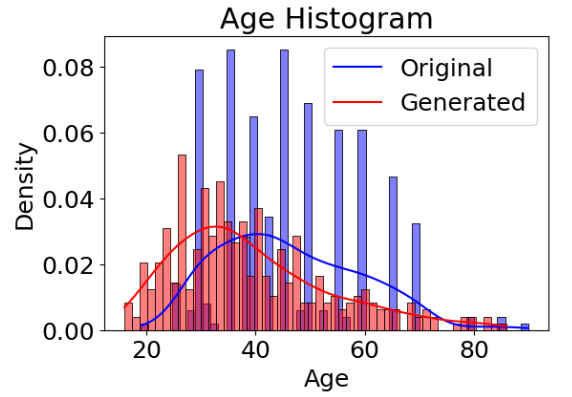
\includegraphics[width=\textwidth]{images/age_ctgan.png}
        \caption{CTGAN}
        \label{fig:age_ctgan}
    \end{subfigure}
    \hfill
    \begin{subfigure}[b]{0.45\textwidth}
        \centering
        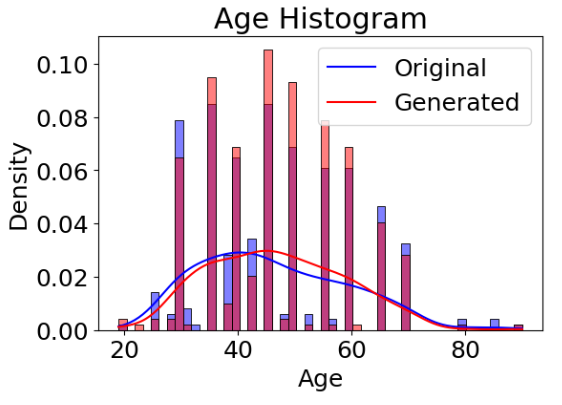
\includegraphics[width=\textwidth]{images/age_begreat.png}
        \caption{BeGreat}
        \label{fig:age_begreat}
    \end{subfigure}
    \hfill
    \begin{subfigure}[b]{0.45\textwidth}
        \centering
        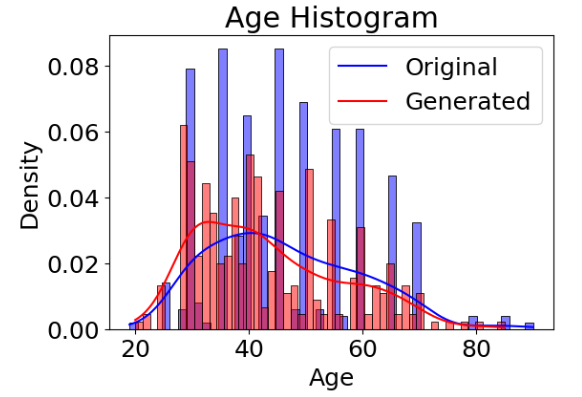
\includegraphics[width=\textwidth]{images/age_llama.png}
        \caption{LLaMa-3}
        \label{fig:age_llama}
    \end{subfigure}
    \caption{Age Distribution for Different Models}
    \label{fig:age_distrib}
\end{figure}

From figure \ref{fig:age_distrib}, the density curve \ref{fig:age_ctgan} shows that the CTGAN model can capture the dominant patient age demographic. Nonetheless, there is a slight variation compared to the original data.
The density curves, from \ref{fig:age_begreat}, indicate an almost perfect alignment between the generated data and the original data, showcasing the model's effectiveness in replicating the age distribution. The density curve from the LLaMa-3 model (\ref{fig:age_llama}) shows a very close alignment with the original data, but it is still better compared to the CTGAN and not as precise as the BeGreat model.


\begin{figure}[H]
    \centering
    \begin{subfigure}[b]{0.45\textwidth}
        \centering
        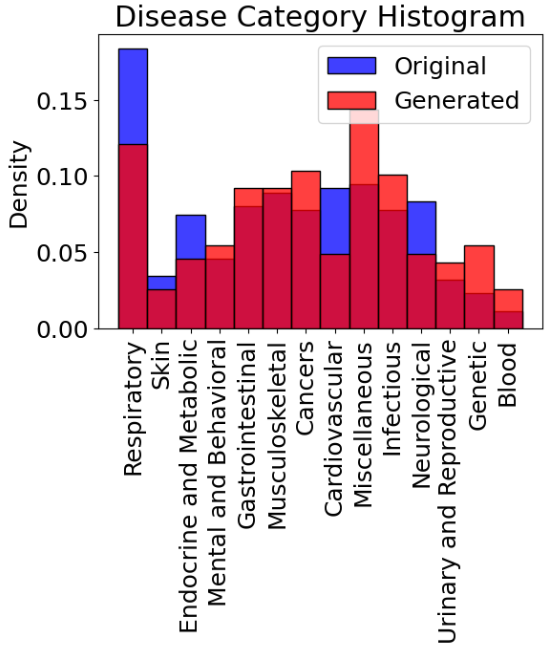
\includegraphics[width=\textwidth]{images/disease_ctgan.png}
        \caption{CTGAN}
        \label{fig:disease_ctgan}
    \end{subfigure}
    \hfill
    \begin{subfigure}[b]{0.45\textwidth}
        \centering
        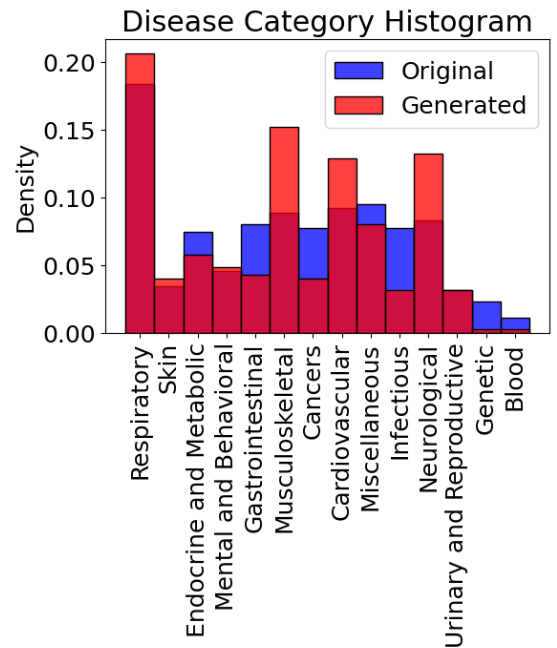
\includegraphics[width=\textwidth]{images/disease_begreat.png}
        \caption{BeGreat}
        \label{fig:disease_begreat}
    \end{subfigure}
    \hfill
    \begin{subfigure}[b]{0.45\textwidth}
        \centering
        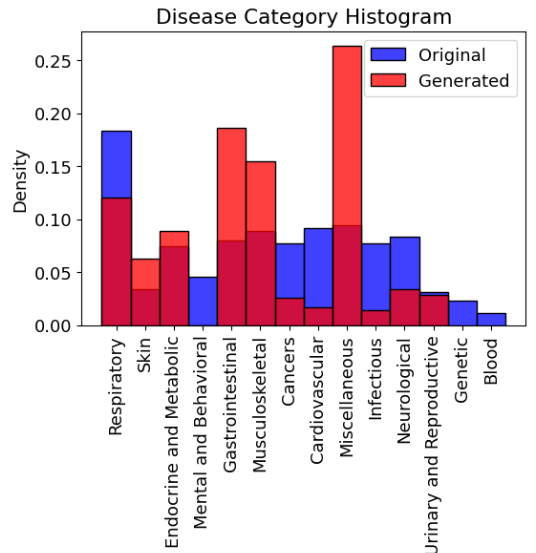
\includegraphics[width=\textwidth]{images/disease_llama.png}
        \caption{LLaMa-3}
        \label{fig:disease_llama}
    \end{subfigure}
    \caption{Comparison of Disease Categories Between Original and Generated Data for Different Models}
    \label{fig:disease_distrib}
\end{figure}

Figure \ref{fig:disease_distrib} illustrates the disease distribution from the original and synthetic data. CTGAN (\ref{fig:disease_ctgan}) as well as BeGreat (\ref{fig:disease_begreat}) replicate almost identical to the original data. However, LLaMa-3 (\ref{fig:disease_llama}) suggests a more different and diverse range of diseases with a high density for the miscellaneous category. LLaMa-3 was given a prompt where was asked the model to generate new diseases, which is why there is a higher density in the miscellaneous category.



%\begin{figure}[H]
%    \centering
%    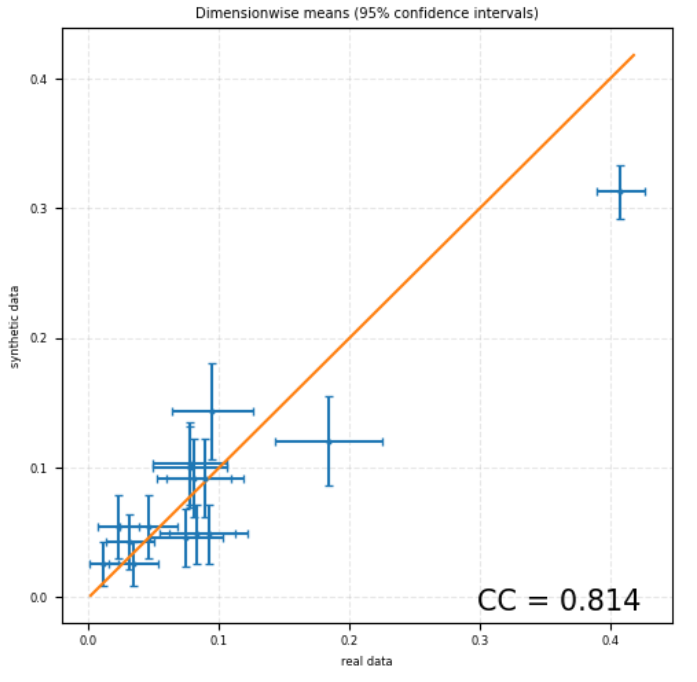
\includegraphics[width=1\linewidth]{images/avg_dim_ctgan.png}
%    \caption{Enter Caption}
%    \label{fig:enter-label}
%    \caption{Mutual Information Matrix Difference for Llama3 Model}
%    \label{fig:llama3_mutual_info}
%\end{figure}

\subsubsection{Summary}



\subsection{Comparative Analysis of Original and Synthetic Data}

\subsubsection{Results}


\begin{figure}[H]
    \centering
    \begin{subfigure}[b]{0.45\textwidth}
        \centering
        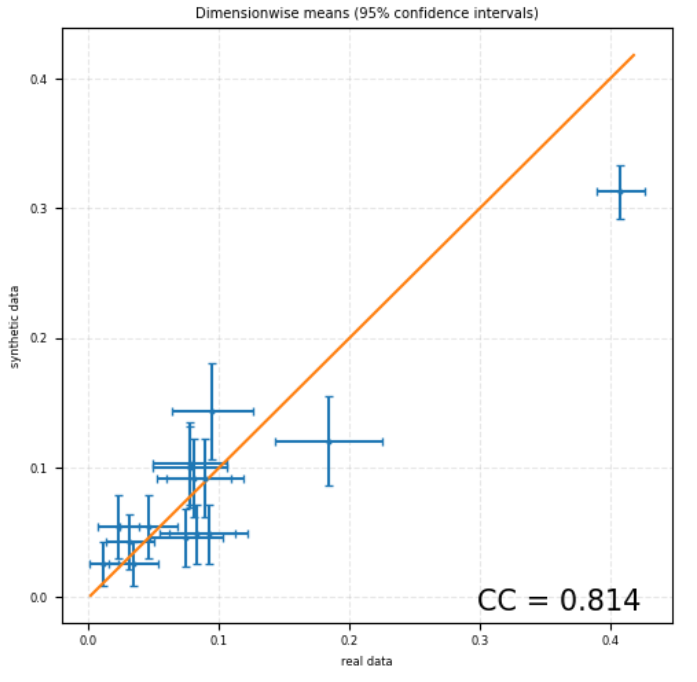
\includegraphics[width=\textwidth]{images/avg_dim_ctgan.png}
        \caption{CTGAN}
        \label{fig:avg_dim_ctgan}
    \end{subfigure}
    \hfill
    \begin{subfigure}[b]{0.45\textwidth}
        \centering
        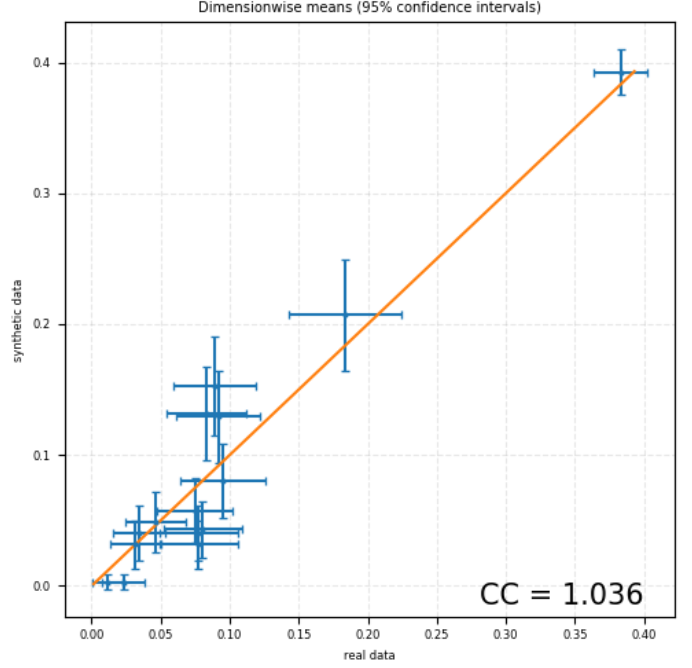
\includegraphics[width=\textwidth]{images/avg_dim_begreat.png}
        \caption{BeGreat}
        \label{fig:avg_dim_begreat}
    \end{subfigure}
    \hfill
    \begin{subfigure}[b]{0.48\textwidth}
        \centering
        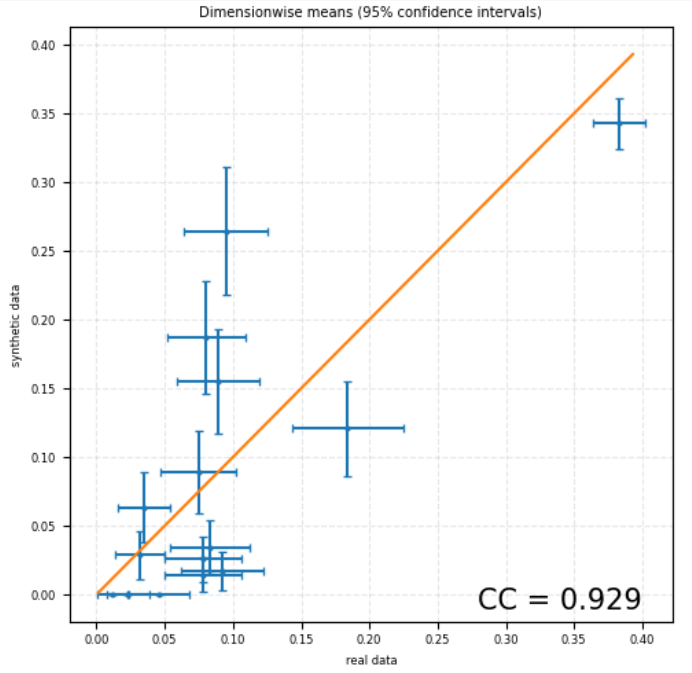
\includegraphics[width=\textwidth]{images/avg_dim_llama.png}
        \caption{LLaMa-3}
        \label{fig:avg_dim_llama}
    \end{subfigure}
    \caption{Dimensionwise means (95\% confidence intervals) scatter plots for different models}
    \label{fig:dim_means_distrib}
\end{figure}

Figure \ref{fig:dim_means_distrib} shows different scatter plots of the dimensionwise means with 95\% confidence intervals. The CTGAN model (\ref{fig:avg_dim_ctgan}) shows a correlation coefficient of 0.814, demonstrating that the model can synthesize correlated data to the original data with a high concentration of points in the lower values. However, the BeGreat model (\ref{fig:avg_dim_begreat}) has a correlation value of 1.036 which shows a perfect correlation between the synthetic and original data. This strong correlation can also be seen in the distribution \ref{fig:age_begreat}. LLaMa-3 has a correlation coefficient of 0.929 (\ref{fig:avg_dim_llama}), indicating that the model could capture the complex distribution of the original data.



\vspace{0.5cm}


\begin{figure}[H]
    \centering
        \centering
        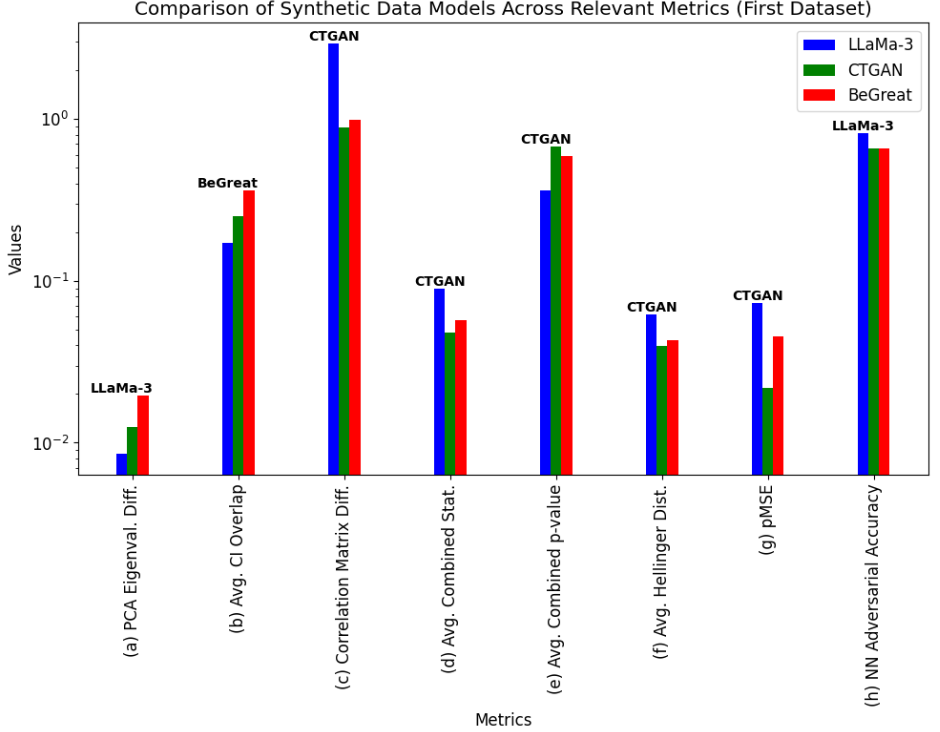
\includegraphics[width=1\textwidth]{images/dataset1_metrics.png}
        \caption{Comparison of synthetic data models across different metrics for the first dataset. In blue, LLaMa-3, in green CTGAN, in red BeGreat.}
        \label{fig:dataset1_metrics}
\end{figure}

\begin{enumerate}
    \item[(a)] PCA Eigenvalue Difference \\
    LLaMa-3 has the lowest PCA Eigenvalue Difference suggesting it best captures the variance of the original data. 

    \item[(b)] Average Confidence Interval Overlap \\
    BeGreat shows the highest average CI overlap indicating its consistency in preserving variability of the original data.

    \item[(c)] Correlation Matrix Difference \\
    CTGAN model preserves better the relationships between variables.

    \item[(d \& e)] Average Combined Statistics \& Average Combined p-value \\
    CTGAN model has the lowest value for the average combined statistics and the highest average combined p-value which both indicate the closest distributional match.

    \item[(f)] Average Hellinger Distance \\
    CTGAN model shows the lowest average Hellinger distance value indicating the closest match to the original data’s distribution.

    \item[(g)] pMSE \\
    CTGAN has low pMSE values, indicating it effectively replicates the original data.

    \item[(h)] NN Adversarial Accuracy \\
    Llama3 shows high adversarial accuracy, indicating variability in distinguishability.
\end{enumerate}

\subsubsection{Summary}

test


\subsection{Classification Accuracy Test Results}

The generated data consists of only 348 individual records, which is considered very low for training and evaluating machine learning models. A small training sample can lead to inaccuracies and biased outcomes. 


\begin{figure}[H]
    \centering
        \centering
        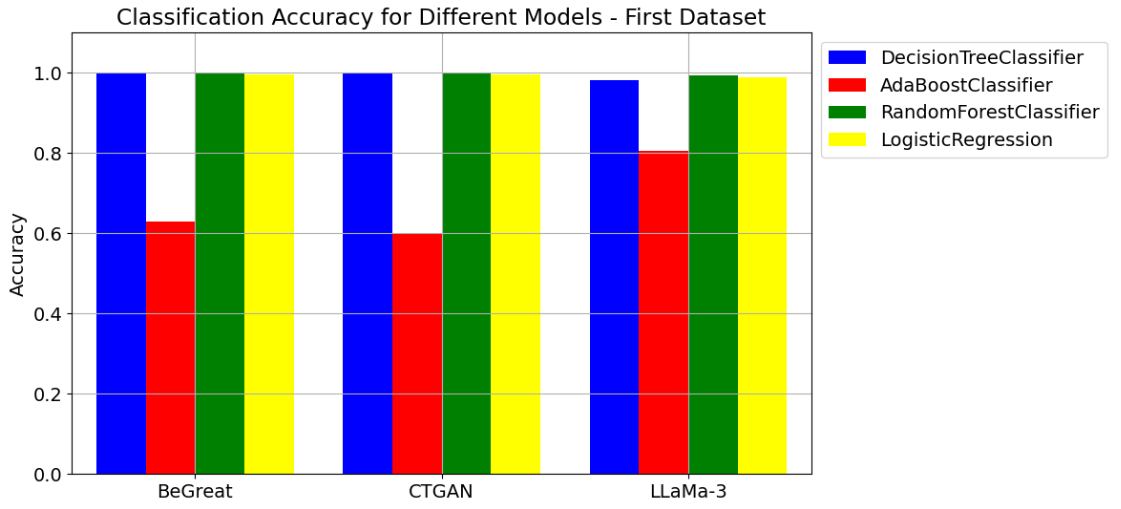
\includegraphics[width=1\textwidth]{images/dataset1_ml.png}
        \caption{Comparison of classification accuracy across machine learning models for the first dataset using Decision Tree Classifier, AdaBoost Classifier, Random Forest Classifier, and Logistic Regression.}
        \label{fig:dataset1_ml}
\end{figure}

Figure \ref{fig:dataset1_ml} shows the performance of different machine learning models using the first dataset. The decision tree, random forest classifiers and the logistic regression all show high accuracies. This is highly due to the fact that the model has been trained on a small sample and cannot give consistent and accurate results. However, the AdaBoost classifier was able to capture the difference lying in the different generated data. LLaMa-3 is outperforming both BeGreat and CTGAN and demonstrates the highest overall accuracies. The same goes for the BeGreat model it was able to perform better than CTGAN.



\subsection{Privacy Metrics Comparison}

For better visualization, the results of the data privacy metrics are normalized. 


\begin{figure}[H]
    \centering
        \centering
        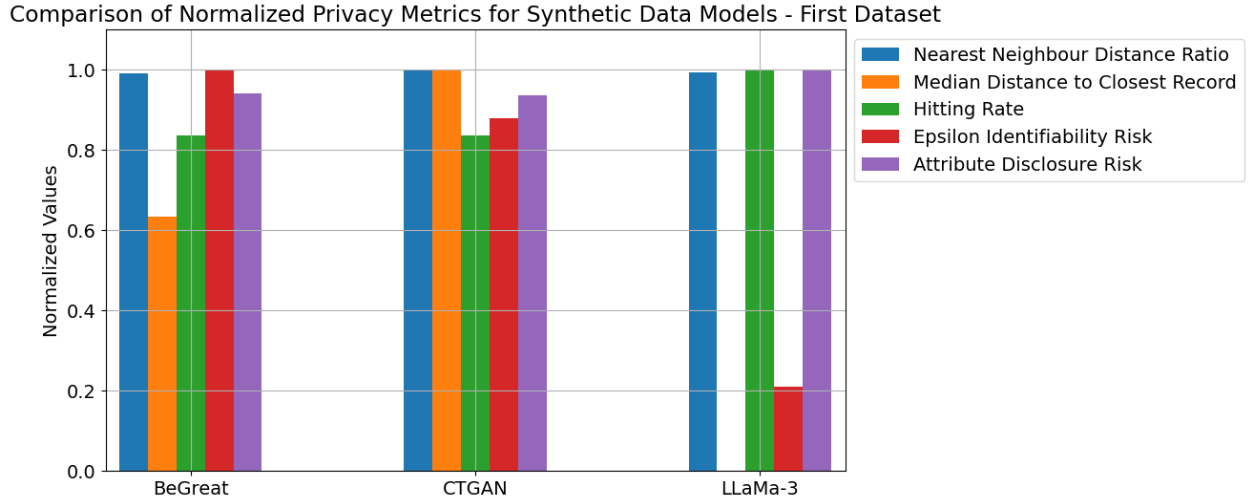
\includegraphics[width=1\textwidth]{images/dataset1_privacy.png}
        \caption{Comparison of normalised privacy metrics for synthetic data models in the first dataset.}
        \label{fig:dataset1_privacy}
\end{figure}

Figure \ref{fig:dataset1_privacy} shows various privacy metrics results of the different models.

\begin{enumerate}
    \item[(a)] Nearest Neighbour Distance Ratio \\
    All models show very close values to 1.0. However, a high value of the neatest neighbour distance ratio indicates a low privacy. Digging into the precise values of the metric, which can be found in the appendix, the BeGreat suggests a lower value compared to the other two models. Nonetheless, data privacy is not respected for all models for that particular metric.

    \item[(b)] Median Distance to Closest Record \\
    CTGAN shows the highest median distance to the closest record, indicating the best privacy. Model BeGreat follows after the CTGAN model, while Model Llama3 has an infinite median distance, suggesting perfect privacy. % need to be checked

    
    \item[(c)] Hitting Rate \\
    LLaMa-3 suggests a higher hitting rate (0.0172), indicating slightly low privacy. BeGreat and CTGAN show the lowest hitting rate (0.0144), indicating better privacy. However, all hitting rates are close to the value 0 which in that case the normalization is not suited for this metric. Thus, all models contribute to better data privacy.


    \item[(d)] Epsilon Identifiability Risk \\
    LLaMa-3 shows the lowest epsilon identifiability risk (0.0805), followed by CTGAN (0.3381). BeGreat has the highest risk (0.3849). CTGAN and BeGreat have almost the same risk value, which suggests lower privacy. On the other hand, LLaMa-3 has a value much closer to 0, indicating that it performs better at generating data with a low risk of exposing real information. 

    \item[(e)] Attribute Disclosure Risk \\
    CTGAN shows the lowest attribute disclosure risk (0.7993), followed closely by BeGreat (0.8044). Llama3 has the highest risk (0.8540), indicating lower privacy. However, all models have a relatively high value of the attribute disclosure risk, which suggests they are as vulnerable as the others. %% better reformulation
    
\end{enumerate}




%%%%%%%%%%%%%%%%%%%%%%%%%%%%%%%%%%%%%%%%%%%%%%%%%%%%%%%%%%%%%%%%%%%%%%%%%%%%%%%%%%%%%%%%%%%%%%%%%%%%%%%%%%%%%%%%%%%%%%%%%%%%%%%%%%%%%%%%%%%%%%%%%%%%%%%%%%%%%%%%%%%%%%%%%%%%%%%%%%%%%%%%%%%%%%%%%%%%%%%%%%%%%%%%%%%%%%%%%%%%%%%%%%%%%%%%%%%%%%%%%%%%%%%%%%%%%%%%%%%%%%%%%%%%%%%%%%%%%%%%%%%%%%%%%%%%%%%%%%%%%%%%%%%%%%%%%%%%%%%%%%%%%%%%%%%%%%%%%%%%%%%%%%%%%%%%%%%%%%%%%%%%%%%%%%%%%%%%%%%%%%%%%%%%%%%%%%%%%%%%%%%%%%%%%%%%%%%%%%%%%%%%%%%%%%%%%%%%%%%%%%%%%%%%%%%%%%%%%%%%



\section{Second Dataset}

\subsection{Statistical Distribution}

\subsection{Comparative Analysis of Original and Synthetic Data}

\begin{figure}[H]
    \centering
    \begin{subfigure}[b]{0.47\textwidth}
        \centering
        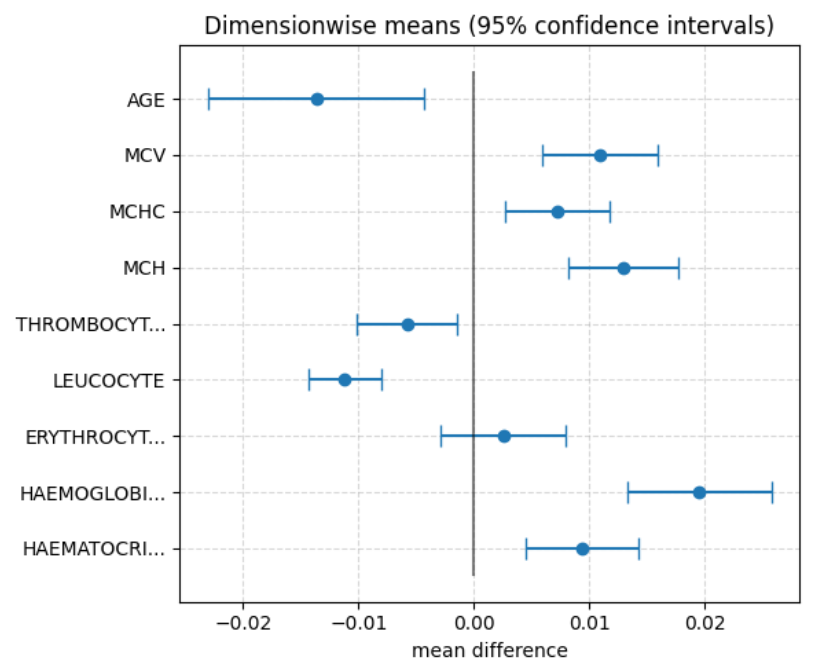
\includegraphics[width=\textwidth]{images/avg_dim_2_ctgan.png}
        \caption{CTGAN}
        \label{fig:avg_dim_2_ctgan}
    \end{subfigure}
    \hfill
    \begin{subfigure}[b]{0.47\textwidth}
        \centering
        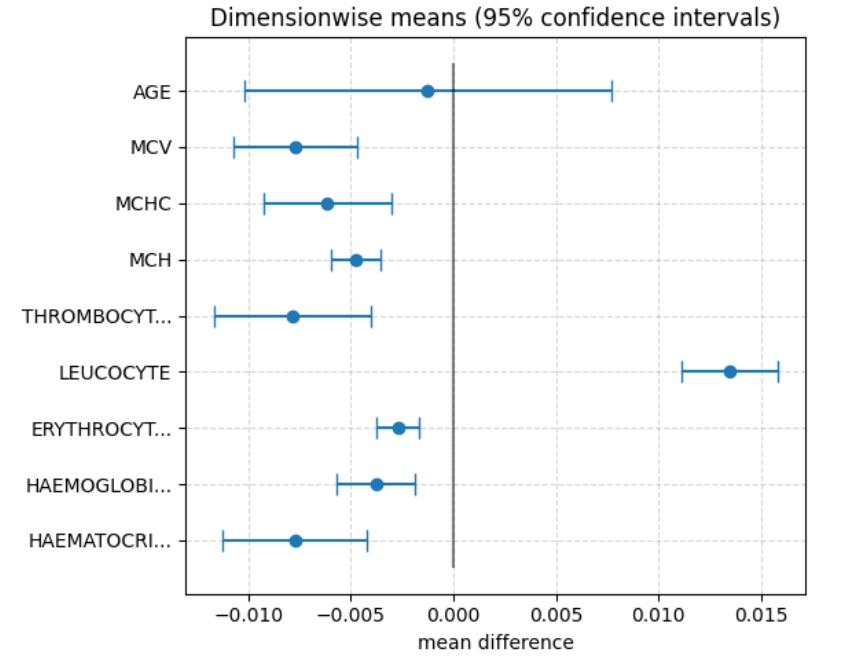
\includegraphics[width=\textwidth]{images/avg_dim_2_begreat.png}
        \caption{BeGreat}
        \label{fig:avg_dim_2_begreat}
    \end{subfigure}
    \hfill
    \begin{subfigure}[b]{0.48\textwidth}
        \centering
        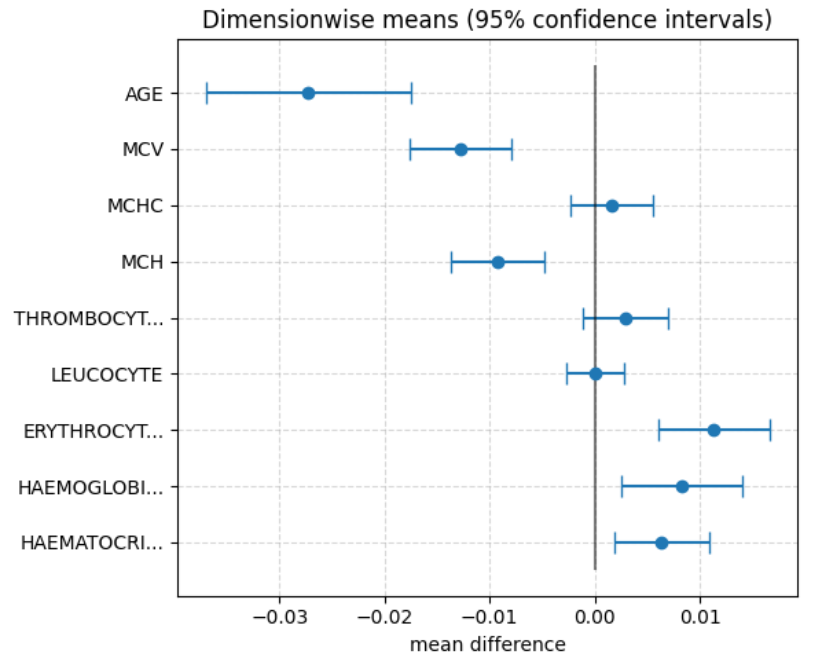
\includegraphics[width=\textwidth]{images/avg_dim_2_llama.png}
        \caption{LLaMa-3}
        \label{fig:avg_dim_2_llama}
    \end{subfigure}
    \caption{Dimensionwise means (95\% confidence intervals) mean-difference plot for different models}
    \label{fig:dim_means_distrib_2}
\end{figure}


Figure \ref{fig:dim_means_distrib_2} shows the mean-difference plots for different models. LLaMa-3 (\ref{fig:avg_dim_2_llama}) shows a drastic shift of the 'AGE' from the zero difference line (black vertical bar) showing that the model tends to generate more variability for the patient's age compared with the original data. On the other hand, the BeGreat model (\ref{fig:avg_dim_2_begreat}) shows a much closer 'AGE' variability from the original data. 
The BeGreat model shows relatively close values from the zero difference line for the other variables indicating that these variables are closer to the real data's variables. Conversely, the CTGAN and the LLaMa-3 model both depict more varied mean differences of variables such as MCV, ERYTHROCYTE etc... leading to more distinct data than the original data. 




\begin{figure}[H]
    \centering
        \centering
        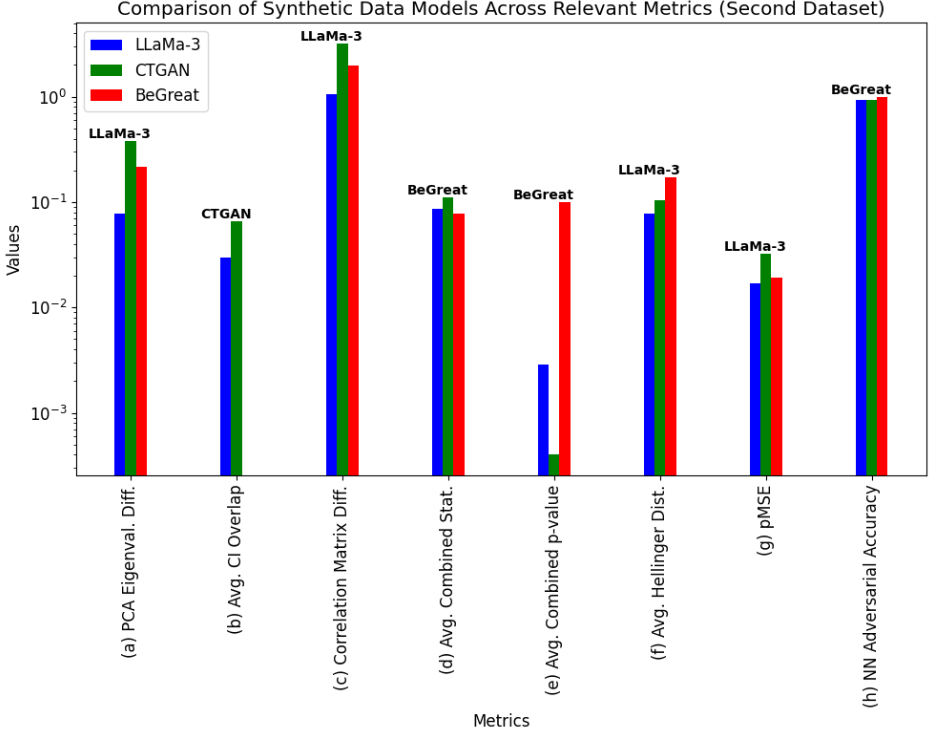
\includegraphics[width=1\textwidth]{images/dataset2_metrics.png}
        \caption{Comparison of synthetic data models across different metrics for the second dataset. In blue, LLaMa-3, in green CTGAN, in red BeGreat.}
        \label{fig:dataset2_metrics}
\end{figure}

\begin{enumerate}
    \item[(a)] PCA Eigenvalue Difference \\
    LLaMa-3 has the lowest PCA Eigenvalue Difference suggesting it best captures the variance of the original data. 

    \item[(b)] Average Confidence Interval Overlap \\
    CTGAN shows the highest average CI overlap indicating its consistency in preserving variability of the original data.

    \item[(c)] Correlation Matrix Difference \\
    LLaMa-3 model preserves better the relationships between variables.

    \item[(d \& e)] Average Combined Statistics \& Average Combined p-value \\
    BeGreat model has the lowest value for the average combined statistics and the highest average combined p-value which both indicate the closest distributional match.

    \item[(f)] Average Hellinger Distance \\
    LLaMa-3 model shows the lowest average Hellinger distance value indicating the closest match to the original data’s distribution.

    \item[(g)] pMSE \\
    LLaMa-3 has low pMSE values, indicating it effectively replicates the original data.

    \item[(h)] NN Adversarial Accuracy \\
    BeGreat shows high adversarial accuracy, indicating variability in distinguishability.
\end{enumerate}

\subsubsection{Summary}

test



\subsection{Classification Accuracy Test Results}




\begin{figure}[H]
    \centering
        \centering
        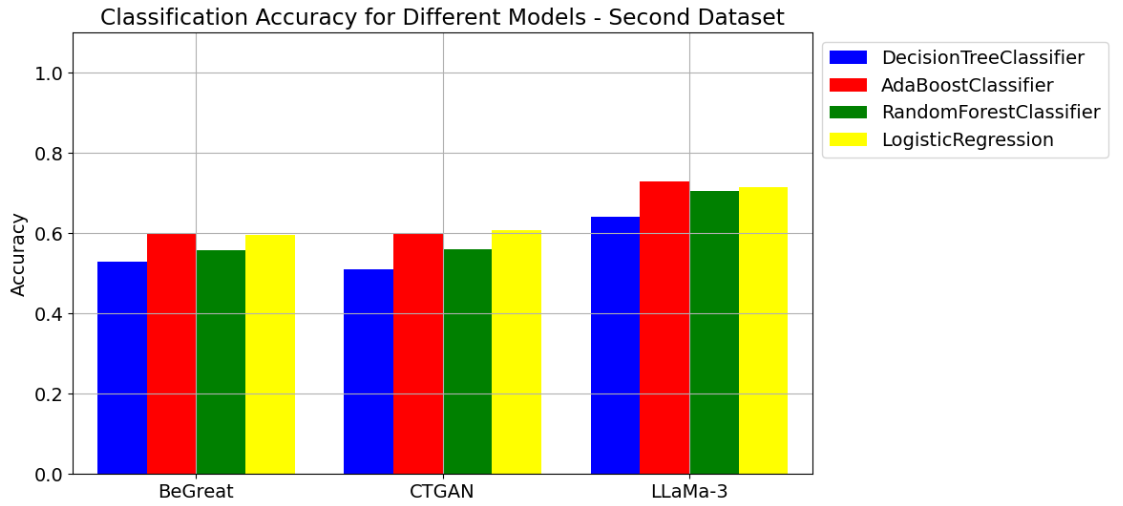
\includegraphics[width=1\textwidth]{images/dataset2_ml.png}
        \caption{Comparison of classification accuracy across machine learning models for the second dataset using Decision Tree Classifier, AdaBoost Classifier, Random Forest Classifier, and Logistic Regression.}
        \label{fig:dataset2_ml}
\end{figure}

Figure \ref{fig:dataset2_ml} shows the performance results of the different machine learning models. It can be observed that CTGAN and the BeGreat model have similar accuracy results. However, the LLaMa-3 model outperforms both the BeGreat and CTGAN models across all machine learning models.





\subsection{Privacy Metrics Comparison}

\begin{figure}[H]
    \centering
        \centering
        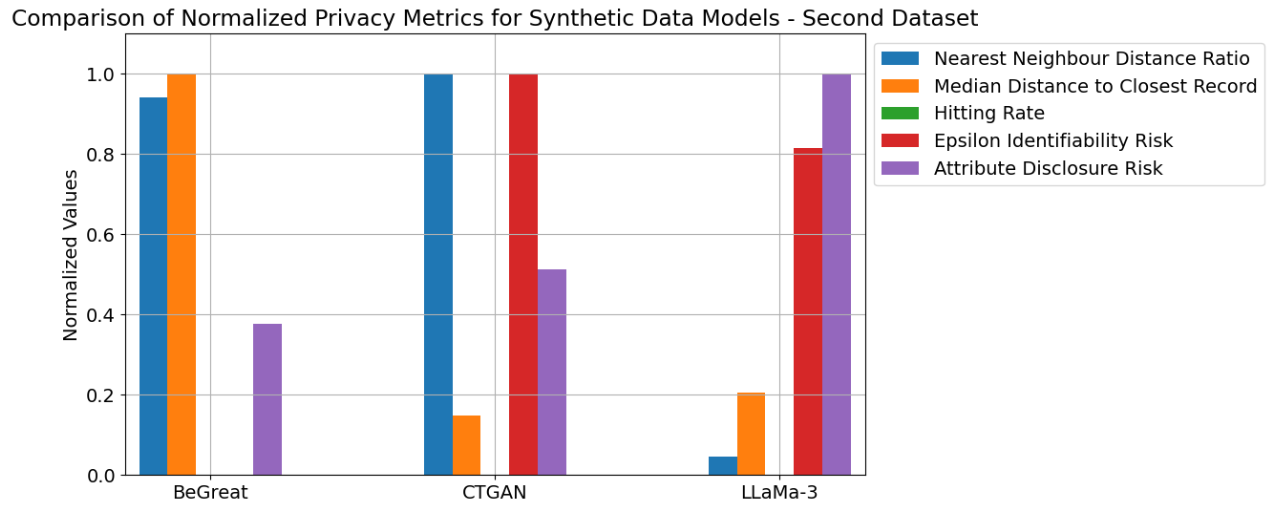
\includegraphics[width=1\textwidth]{images/dataset2_privacy.png}
        \caption{Comparison of normalised privacy metrics for synthetic data models in the second dataset.}
        \label{fig:dataset2_privacy}
\end{figure}


\begin{enumerate}
    \item[(a)] Nearest Neighbour Distance Ratio \\
    The CTGAN model exhibits the highest value among the other models, this suggests a closer generated data to the real data which tends to lower the privacy. On the other hand, the LLaMa-3 model shows a much lower value for this metric suggesting better privacy preservation in terms of distance from real data.

    \item[(b)] Median Distance to Closest Record \\
    CTGAN shows the lowest median distance to the closest record, indicating that the synthetic data is very close to the real data, which might raise privacy concerns. However, both BeGreat and LLaMa-3 have higher values suggesting perfect privacy.

    
    \item[(c)] Hitting Rate \\
    However, all hitting rates are close to the value 0 which indicates that all models contribute to better privacy.


    \item[(d)] Epsilon Identifiability Risk \\
    BeGreat shows the lowest epsilon identifiability risk (0.0002), followed by LLaMa-3 (0.1729). CTGAN has the highest risk (0.2122). CTGAN and LLaMa-3 have around the same risk value, which suggests lower privacy. On the other hand, BeGreat has a value much closer to 0, indicating that it performs better at generating data with a low risk of exposing real information. 

    \item[(e)] Attribute Disclosure Risk \\
    BeGreat shows the lowest attribute disclosure risk, followed closely by CTGAN. LLaMa-3 has the highest risk, indicating lower privacy. However, all models have a relatively high value of the attribute disclosure risk, which suggests they are as vulnerable as the others. %% better reformulation
    
\end{enumerate}















\vspace{10cm}




\section{Comparative Analysis of Original and Synthetic Data}

\subsection{Average Dimensionwise Means Difference}

\begin{table}[H]
\centering
\caption{Average Dimensionwise Means Difference for Synthetic Data Models}
\label{tab:avg_means_diff_combined}
\begin{tabularx}{\textwidth}{l*{6}{X}}
    \toprule
    \textbf{Model} & \multicolumn{3}{c}{\textbf{First Data}} & \multicolumn{3}{c}{\textbf{Second Data}} \\
    \cmidrule(lr){2-4} \cmidrule(lr){5-7}
    & \textbf{Llama3} & \textbf{CTGAN} & \textbf{BeGreat} & \textbf{Llama3} & \textbf{CTGAN} & \textbf{BeGreat} \\
    \midrule
    Avg. Means Diff. & 0.0586 ± 0.0062 & 0.0281 ± 0.0052 & 0.0325 ± 0.0051 & 0.0266 ± 0.0009 & 0.0232 ± 0.0010 & 0.0170 ± 0.0007 \\
    \bottomrule
\end{tabularx}
\end{table}



From Table \ref{tab:avg_means_diff_combined}, we can analyze the performance of each model across both data sets:

\textbf{BeGreat} has the smallest mean difference in both data sets, indicating it most accurately replicates the average values of the original data.
\textbf{CTGAN} follows closely, showing slightly higher average means differences but still demonstrating good accuracy.
\textbf{Llama3} has the largest mean difference in both data sets but still maintains a reasonable level of accuracy.

\vspace{0.5cm}


The comparison of average dimensionwise means differences reveals that:

\textbf{BeGreat} consistently provides the best performance in terms of replicating the original data's mean values across both data sets.
\textbf{CTGAN} also performs well, showing small differences in average means but slightly larger than BeGreat.
\textbf{Llama3} shows the largest differences but remains within an acceptable range of accuracy.


\vspace{0.5cm}

These findings highlight the strengths of each model in replicating the original data's mean values. The BeGreat model is recommended for applications requiring the highest fidelity in replicating mean values, while the CTGAN model offers a balanced performance. The Llama3 model, although showing slightly larger differences, still provides reasonable accuracy and may be suitable for applications with less stringent requirements on mean value replication.




\subsection{PCA Metrics}

\begin{table}[H]
\centering
\caption{PCA Metrics for Synthetic Data Models}
\label{tab:pca_metrics_combined}
\begin{tabularx}{\textwidth}{l*{6}{X}}
    \toprule
    \textbf{Metric Description} & \multicolumn{3}{c}{\textbf{First Data}} & \multicolumn{3}{c}{\textbf{Second Data}} \\
    \cmidrule(lr){2-4} \cmidrule(lr){5-7}
    & \textbf{Llama3} & \textbf{CTGAN} & \textbf{BeGreat} & \textbf{Llama3} & \textbf{CTGAN} & \textbf{BeGreat} \\
    \midrule
    PCA Eigenval. Diff. & 0.0085 & 0.0125 & 0.0196 & 0.0781 & 0.3825 & 0.2181 \\
    PCA Eigenvec. Angle & 1.0226 & 0.9035 & 1.5565 & 0.9489 & 1.5186 & 0.2738 \\
    \bottomrule
\end{tabularx}
\end{table}


From Table \ref{tab:pca_metrics_combined}, the PCA metrics evaluate how well the synthetic data captures the variance and structure of the original data:

\textbf{Llama3} consistently shows the smallest eigenvalue difference in both datasets, indicating it best captures the variance of the original data.
\textbf{BeGreat} excels in preserving the structural similarity in the second dataset but not as well in the first dataset.
\textbf{CTGAN} shows the largest differences in both metrics in the second dataset but performs better in the first dataset, particularly in preserving structural similarity.

\vspace{0.5cm}

The comparison of PCA metrics reveals that:

\textbf{Llama3} consistently provides the best performance in terms of capturing the variance of the original data across both datasets.
\textbf{BeGreat} shows a strong performance in preserving structural similarity in the second dataset but less so in the first dataset.
\textbf{CTGAN} performs well in the first dataset but shows larger differences in the second dataset, indicating variability in its effectiveness.

\vspace{0.5cm}

These findings highlight the strengths and limitations of each model in terms of PCA metrics. The Llama3 model is recommended for applications requiring high fidelity in capturing the variance of the original data, while the BeGreat model offers strong performance in preserving structural similarity in certain cases. The CTGAN model, while showing good performance in some cases, may require further refinement for consistent results.








\subsection{Confidence Interval Overlap}

\begin{table}[H]
\centering
\caption{Confidence Interval Overlap for Synthetic Data Models}
\label{tab:ci_overlap_combined}
\begin{tabularx}{\textwidth}{l*{6}{X}}
    \toprule
    \textbf{Metric Description} & \multicolumn{3}{c}{\textbf{First Data}} & \multicolumn{3}{c}{\textbf{Second Data}} \\
    \cmidrule(lr){2-4} \cmidrule(lr){5-7}
    & \textbf{Llama3} & \textbf{CTGAN} & \textbf{BeGreat} & \textbf{Llama3} & \textbf{CTGAN} & \textbf{BeGreat} \\
    \midrule
    Avg. CI Overlap & 0.1725 ± 0.1038 & 0.2497 ± 0.0805 & 0.3632 ± 0.0996 & 0.0300 ± 0.0300 & 0.0654 ± 0.0437 & 0.0000 ± 0.0000 \\
    \# Non-overlapping CIs & 9 & 7 & 7 & 8 & 7 & 9 \\
    Frac. Non-overlapping CIs & 0.7500 & 0.4667 & 0.4667 & 0.8889 & 0.7778 & 1.0000 \\
    \bottomrule
\end{tabularx}
\end{table}



From Table \ref{tab:ci_overlap_combined}, the confidence interval overlap measures how well the variability in the synthetic data matches the original data:

\textbf{BeGreat} shows no overlap in the second dataset but the highest average CI overlap in the first dataset, indicating inconsistency in preserving variability.
\textbf{CTGAN} performs well in both datasets, showing the highest average CI overlap in the second dataset and a strong performance in the first dataset.
\textbf{Llama3} shows moderate performance in both datasets, with lower average CI overlap compared to CTGAN and BeGreat.

\vspace{0.5cm}

The comparison of confidence interval overlap reveals that:

\textbf{CTGAN} consistently provides good performance in terms of preserving variability across both datasets.
\textbf{BeGreat} shows strong performance in the first dataset but no overlap in the second dataset, indicating variability in its effectiveness.
\textbf{Llama3} shows moderate performance in both datasets but generally lower average CI overlap compared to CTGAN and BeGreat.

\vspace{0.5cm}

These findings highlight the strengths and limitations of each model in terms of confidence interval overlap. The CTGAN model is recommended for applications requiring consistent preservation of variability, while the BeGreat model offers strong performance in some cases. Although the Llama3 model shows moderate performance, it may be suitable for applications with less stringent requirements for variability preservation.





\subsection{Correlation Metrics}

\begin{table}[H]
\centering
\caption{Correlation Metrics for Synthetic Data Models}
\label{tab:correlation_metrics_combined}
\begin{tabularx}{\textwidth}{l*{6}{X}}
    \toprule
    \textbf{Metric Description} & \multicolumn{3}{c}{\textbf{First Data}} & \multicolumn{3}{c}{\textbf{Second Data}} \\
    \cmidrule(lr){2-4} \cmidrule(lr){5-7}
    & \textbf{Llama3} & \textbf{CTGAN} & \textbf{BeGreat} & \textbf{Llama3} & \textbf{CTGAN} & \textbf{BeGreat} \\
    \midrule
    Correlation Matrix Diff. & 2.9316 & 0.8911 & 0.9849 & 1.0608 & 3.2077 & 1.9991 \\
    Mutual Info. Diff. & 2.7911 & 0.6086 & 0.5918 & 0.1937 & 0.2485 & 1.1123 \\
    \bottomrule
\end{tabularx}
\end{table}




From Table \ref{tab:correlation_metrics_combined}, correlation metrics assess the preservation of relationships between variables:

\textbf{Llama3} consistently shows the smallest differences in both correlation metrics across both datasets, indicating it best preserves the relationships between variables.
\textbf{CTGAN} shows larger differences in the second dataset but performs reasonably well in the first dataset.
\textbf{BeGreat} has the largest differences in mutual information in the second dataset and a missing value for the correlation matrix difference in the first dataset, indicating variability in its effectiveness.

\vspace{0.5cm}

The comparison of correlation metrics reveals that:

\textbf{Llama3} consistently provides the best performance in terms of preserving relationships between variables across both datasets.
\textbf{CTGAN} performs well in the first dataset but shows larger differences in the second dataset, indicating variability in its effectiveness.
\textbf{BeGreat} shows the largest differences in mutual information in the second dataset and has inconsistent results in the first dataset.

\vspace{0.5cm}

These findings highlight the strengths and limitations of each model in terms of correlation metrics. The Llama3 model is recommended for applications requiring high fidelity in preserving relationships between variables, while the CTGAN model offers reasonable performance in some cases. The BeGreat model, although showing some inconsistencies, may still be suitable for certain applications with less stringent requirements on preserving relationships.








\subsection{Kolmogorov-Smirnov / Total Variation Distance Test}



\begin{table}[H]
\centering
\caption{Kolmogorov-Smirnov / Total Variation Distance Test for Synthetic Data Models}
\label{tab:ks_tv_test_combined}
\begin{tabularx}{\textwidth}{l*{6}{X}}
    \toprule
    \textbf{Metric Description} & \multicolumn{3}{c}{\textbf{First Data}} & \multicolumn{3}{c}{\textbf{Second Data}} \\
    \cmidrule(lr){2-4} \cmidrule(lr){5-7}
    & \textbf{Llama3} & \textbf{CTGAN} & \textbf{BeGreat} & \textbf{Llama3} & \textbf{CTGAN} & \textbf{BeGreat} \\
    \midrule
    Avg. Combined Stat. & 0.0894 ± 0.0185 & 0.0478 ± 0.0120 & 0.0573 ± 0.0118 & 0.0863 ± 0.0174 & 0.1110 ± 0.0201 & 0.0781 ± 0.0140 \\
    Avg. KS Dist. & 0.0699 ± 0.0167 & 0.0426 ± 0.0159 & 0.0400 ± 0.0126 & 0.0974 ± 0.0193 & 0.0946 ± 0.0196 & 0.0936 ± 0.0117 \\
    Avg. TV Dist. & 0.1089 ± 0.0330 & 0.0565 ± 0.0186 & 0.0860 ± 0.0207 & 0.0362 ± 0.0121 & 0.1848 ± 0.0404 & 0.0087 ± 0.0080 \\
    Avg. Combined p-value & 0.3600 ± 0.0858 & 0.6765 ± 0.0812 & 0.5865 ± 0.0850 & 0.0029 ± 0.0027 & 0.0004 ± 0.0003 & 0.1006 ± 0.0887 \\
    \# Sig. Tests (\(\alpha=0.05\)) & 9 & 2 & 6 & 11 & 11 & 9 \\
    Frac. Sig. Tests & 0.3750 & 0.0833 & 0.2500 & 1.0000 & 1.0000 & 0.8182 \\
    \bottomrule
\end{tabularx}
\end{table}



From Table \ref{tab:ks_tv_test_combined}, the Kolmogorov-Smirnov (KS) and Total Variation (TV) distance tests evaluate the distributional similarity between synthetic and original data:

\textbf{BeGreat} consistently shows the smallest combined statistics and high p-values across both datasets, indicating the closest distributional match.
\textbf{Llama3} performs well, with moderate combined statistics and reasonable p-values, indicating a good distributional match.
\textbf{CTGAN} shows larger combined statistics and more significant tests in the second dataset but performs better in the first dataset, indicating variability in its effectiveness.

\vspace{0.5cm}

The comparison of KS and TV distance tests reveals that:

\textbf{BeGreat} consistently provides the best performance in terms of distributional similarity across both datasets.
\textbf{Llama3} shows good performance, with moderate combined statistics and reasonable p-values.
\textbf{CTGAN} shows variability in performance, with larger differences in the second dataset but better results in the first dataset.

\vspace{0.5cm}

These findings highlight the strengths and limitations of each model in terms of distributional similarity. The BeGreat model is recommended for applications requiring the highest fidelity in replicating the original data's distribution, while the Llama3 model offers good performance. Although the CTGAN model shows some variability, it may still be suitable for certain applications.






\subsection{Empirical Hellinger Distance}


\begin{table}[H]
\centering
\caption{Empirical Hellinger Distance for Synthetic Data Models}
\label{tab:hellinger_distance_combined}
\begin{tabularx}{\textwidth}{l*{6}{X}}
    \toprule
    \textbf{Metric Description} & \multicolumn{3}{c}{\textbf{First Data}} & \multicolumn{3}{c}{\textbf{Second Data}} \\
    \cmidrule(lr){2-4} \cmidrule(lr){5-7}
    & \textbf{Llama3} & \textbf{CTGAN} & \textbf{BeGreat} & \textbf{Llama3} & \textbf{CTGAN} & \textbf{BeGreat} \\
    \midrule
    Avg. Hellinger Dist. & 0.0621 ± 0.0243 & 0.0396 ± 0.0228 & 0.0429 ± 0.0160 & 0.0775 ± 0.0288 & 0.1045 ± 0.0252 & 0.1714 ± 0.0636 \\
    \bottomrule
\end{tabularx}
\end{table}



From Table \ref{tab:hellinger_distance_combined}, the empirical Hellinger distance measures the similarity between probability distributions of the original and synthetic data:

\textbf{Llama3} consistently shows the smallest Hellinger distances across both datasets, indicating the closest match to the original data's distribution.
\textbf{CTGAN} follows closely in both datasets, showing slightly larger distances but still a reasonable match.
\textbf{BeGreat} shows the largest distances in both datasets, indicating less similarity in distribution compared to the other models.

\vspace{0.5cm}

The comparison of empirical Hellinger distances reveals that:

\textbf{Llama3} consistently provides the best performance in terms of distributional similarity across both datasets.
\textbf{CTGAN} shows good performance, with slightly larger distances but still maintaining a reasonable match to the original data's distribution.
\textbf{BeGreat} shows the largest distances in both datasets, indicating less similarity in distribution.

\vspace{0.5cm}

These findings highlight the strengths and limitations of each model in terms of empirical Hellinger distance. The Llama3 model is recommended for applications requiring the highest fidelity in replicating the original data's distribution, while the CTGAN model offers good performance. The BeGreat model, although showing larger distances, may still be suitable for certain applications.








\subsection{Propensity Mean Squared Error (pMSE)}


\begin{table}[H]
\centering
\caption{Propensity Mean Squared Error (pMSE) for Synthetic Data Models}
\label{tab:pmse_combined}
\begin{tabularx}{\textwidth}{l*{6}{X}}
    \toprule
    \textbf{Metric Description} & \multicolumn{3}{c}{\textbf{First Data}} & \multicolumn{3}{c}{\textbf{Second Data}} \\
    \cmidrule(lr){2-4} \cmidrule(lr){5-7}
    & \textbf{Llama3} & \textbf{CTGAN} & \textbf{BeGreat} & \textbf{Llama3} & \textbf{CTGAN} & \textbf{BeGreat} \\
    \midrule
    pMSE & 0.0730 ± 0.0042 & 0.0219 ± 0.0010 & 0.0455 ± 0.0033 & 0.0168 ± 0.0004 & 0.0324 ± 0.0006 & 0.0194 ± 0.0005 \\
    Avg. pMSE Accuracy & 0.7261 ± 0.0196 & 0.5799 ± 0.0147 & 0.6523 ± 0.0206 & 0.5442 ± 0.0072 & 0.6434 ± 0.0072 & 0.5821 ± 0.0072 \\
    \bottomrule
\end{tabularx}
\end{table}



From Table \ref{tab:pmse_combined}, the propensity mean squared error (pMSE) evaluates how well the synthetic data mimics the original data for predictive modeling:

\textbf{Llama3} consistently shows low pMSE values, indicating it effectively replicates the original data.
\textbf{CTGAN} shows variability, with the lowest pMSE in the first dataset but higher pMSE in the second dataset. It also shows the highest average pMSE classifier accuracy in the second dataset.
\textbf{BeGreat} shows higher pMSE values in both datasets but maintains high average pMSE classifier accuracy in the first dataset.

\vspace{0.5cm}

The comparison of pMSE reveals that:

\textbf{Llama3} consistently provides low pMSE values across both datasets, indicating strong performance in replicating the original data.
\textbf{CTGAN} shows variability in pMSE values but performs well in terms of average pMSE classifier accuracy.
\textbf{BeGreat} shows higher pMSE values but maintains high predictive accuracy in the first dataset.

\vspace{0.5cm}

These findings highlight the strengths and limitations of each model in terms of pMSE. The Llama3 model is recommended for applications requiring consistent replication of the original data. The CTGAN model, while showing some variability, offers strong predictive accuracy. The BeGreat model, despite higher pMSE values, may still be suitable for applications prioritizing predictive accuracy.







\subsection{Nearest Neighbour Adversarial Accuracy}


\begin{table}[H]
\centering
\caption{Nearest Neighbour Adversarial Accuracy for Synthetic Data Models}
\label{tab:nn_accuracy_combined}
\begin{tabularx}{\textwidth}{l*{6}{X}}
    \toprule
    \textbf{Metric Description} & \multicolumn{3}{c}{\textbf{First Data}} & \multicolumn{3}{c}{\textbf{Second Data}} \\
    \cmidrule(lr){2-4} \cmidrule(lr){5-7}
    & \textbf{Llama3} & \textbf{CTGAN} & \textbf{BeGreat} & \textbf{Llama3} & \textbf{CTGAN} & \textbf{BeGreat} \\
    \midrule
    NN Adversarial Accuracy & 0.8170 ± 0.0000 & 0.6585 ± 0.0000 & 0.6574 ± 0.0000 & 0.9280 ± 0.0000 & 0.9276 ± 0.0000 & 0.9999 ± 0.0000 \\
    \bottomrule
\end{tabularx}
\end{table}

From Table \ref{tab:nn_accuracy_combined}, the nearest neighbour adversarial accuracy assesses the distinguishability between synthetic and original data:

\textbf{Llama3} shows consistently high adversarial accuracy in the second dataset but lower accuracy in the first dataset, indicating variability in distinguishability.
\textbf{CTGAN} shows similar trends with high accuracy in the second dataset but lower accuracy in the first dataset.
\textbf{BeGreat} shows very high accuracy in the second dataset, suggesting easy distinguishability, and maintains the highest accuracy in the first dataset as well.

\vspace{0.5cm}

The comparison of nearest neighbour adversarial accuracy reveals that:

\textbf{Llama3} produces synthetic data that is harder to distinguish from the original in the second dataset but not as effectively in the first dataset.
\textbf{CTGAN} shows similar performance to Llama3 with high accuracy in the second dataset and lower in the first dataset.
\textbf{BeGreat} shows high accuracy in both datasets, indicating its synthetic data is easier to distinguish from the original.

\vspace{0.5cm}

These findings highlight the strengths and limitations of each model in terms of nearest neighbour adversarial accuracy. The Llama3 and CTGAN models are recommended for applications requiring synthetic data that is hard to distinguish from the original, particularly in the second dataset. The BeGreat model, although showing higher distinguishability, may still be suitable for certain applications with less stringent requirements on indistinguishability or where the primary focus is on other metrics such as distributional similarity or predictive accuracy.




\section{Classification Accuracy Test Results}

\subsection{DecisionTreeClassifier}

\begin{table}[H]
\centering
\caption{Classification Accuracy for DecisionTreeClassifier}
\label{tab:decision_tree_accuracy_combined}
\begin{tabularx}{\textwidth}{l*{8}{X}}
    \toprule
    \textbf{Model} & \multicolumn{3}{c}{\textbf{First Data}} & \multicolumn{4}{c}{\textbf{Second Data}} \\
    \cmidrule(lr){2-4} \cmidrule(lr){5-8}
    & \textbf{Acc\textsubscript{R}} & \textbf{Acc\textsubscript{F}} & \textbf{$|$Diff$|$} & \textbf{Error} & \textbf{Acc\textsubscript{R}} & \textbf{Acc\textsubscript{F}} & \textbf{$|$Diff$|$} & \textbf{Error} \\
    \midrule
    BeGreat & 1.0000 & 0.9818 & 0.0182 & 0.0115 & 0.5300 & 0.5241 & 0.0059 & 0.0117 \\
    CTGAN & 1.0000 & 1.0000 & 0.0000 & 0.0000 & 0.5105 & 0.5079 & 0.0026 & 0.0152 \\
    Llama3 & 0.9820 & 1.0000 & 0.0180 & 0.0113 & 0.6421 & 0.5834 & 0.0586 & 0.0299 \\
    \bottomrule
\end{tabularx}
\end{table}


From Table \ref{tab:decision_tree_accuracy_combined}, the DecisionTreeClassifier is evaluated across different models to measure the classification accuracy on real and synthetic data:

\textbf{CTGAN} shows no difference (0.0000) between real and synthetic data in the first dataset, indicating excellent performance. It also has the smallest accuracy difference (0.0026) in the second dataset, indicating good performance.
\textbf{BeGreat} follows with a difference of 0.0182 in the first dataset and 0.0059 in the second dataset, indicating reasonable accuracy.
\textbf{Llama3} shows the largest difference (0.0180) in the first dataset and the largest difference (0.0586) in the second dataset, though all models demonstrate reasonable accuracy.

\vspace{0.5cm}

The comparison of classification accuracy for DecisionTreeClassifier reveals that:

\textbf{CTGAN} consistently provides the best performance in terms of classification accuracy across both datasets.
\textbf{BeGreat} follows closely, showing small differences in classification accuracy but still performing well.
\textbf{Llama3} shows the largest differences but remains within an acceptable range of accuracy.

\vspace{0.5cm}

These findings highlight the strengths and limitations of each model in terms of classification accuracy for DecisionTreeClassifier. The CTGAN model is recommended for applications requiring the highest classification accuracy. The BeGreat model offers strong performance with slightly larger differences. The Llama3 model, although showing larger differences, still provides reasonable accuracy and may be suitable for applications with less stringent requirements on classification accuracy.





\subsection{AdaBoostClassifier}

\begin{table}[H]
\centering
\caption{Classification Accuracy for AdaBoostClassifier}
\label{tab:adaboost_accuracy_combined}
\begin{tabularx}{\textwidth}{l*{8}{X}}
    \toprule
    \textbf{Model} & \multicolumn{3}{c}{\textbf{First Data}} & \multicolumn{4}{c}{\textbf{Second Data}} \\
    \cmidrule(lr){2-4} \cmidrule(lr){5-8}
    & \textbf{Acc\textsubscript{R}} & \textbf{Acc\textsubscript{F}} & \textbf{$|$Diff$|$} & \textbf{Error} & \textbf{Acc\textsubscript{R}} & \textbf{Acc\textsubscript{F}} & \textbf{$|$Diff$|$} & \textbf{Error} \\
    \midrule
    BeGreat & 0.6295 & 0.5322 & 0.0973 & 0.0579 & 0.6001 & 0.5267 & 0.0734 & 0.0335 \\
    CTGAN & 0.6006 & 0.6008 & 0.0002 & 0.0427 & 0.6006 & 0.4688 & 0.1318 & 0.0153 \\
    Llama3 & 0.8059 & 0.7401 & 0.0658 & 0.0617 & 0.7285 & 0.6661 & 0.0624 & 0.0585 \\
    \bottomrule
\end{tabularx}
\end{table}



From Table \ref{tab:adaboost_accuracy_combined}, the AdaBoostClassifier is evaluated across different models to measure the classification accuracy on real and synthetic data:

\textbf{CTGAN} shows the smallest accuracy difference (0.0002) in the first dataset, indicating excellent performance. It has the largest accuracy difference (0.1318) in the second dataset, suggesting it struggles with the synthetic data in that case.
\textbf{Llama3} follows closely with a difference of 0.0658 in the first dataset and 0.0624 in the second dataset, indicating good performance on synthetic data.
\textbf{BeGreat} has the largest difference (0.0973) in the first dataset and a difference of 0.0734 in the second dataset, indicating it struggles more with the synthetic data.

\vspace{0.5cm}

The comparison of classification accuracy for AdaBoostClassifier reveals that:

\textbf{CTGAN} consistently provides the best performance in terms of classification accuracy in the first dataset but struggles in the second dataset.
\textbf{Llama3} offers strong performance with small differences in classification accuracy across both datasets.
\textbf{BeGreat} shows larger differences but still performs reasonably well in some cases.

\vspace{0.5cm}

These findings highlight the strengths and limitations of each model in terms of classification accuracy for AdaBoostClassifier. The CTGAN model is recommended for applications requiring the highest classification accuracy in the first dataset but may need improvement for other datasets. The Llama3 model offers good performance across both datasets. The BeGreat model, although showing larger differences, may still be suitable for certain applications with less stringent requirements on classification accuracy.










\subsection{RandomForestClassifier}

\begin{table}[H]
\centering
\caption{Classification Accuracy for RandomForestClassifier}
\label{tab:random_forest_accuracy_combined}
\begin{tabularx}{\textwidth}{l*{8}{X}}
    \toprule
    \textbf{Model} & \multicolumn{3}{c}{\textbf{First Data}} & \multicolumn{4}{c}{\textbf{Second Data}} \\
    \cmidrule(lr){2-4} \cmidrule(lr){5-8}
    & \textbf{Acc\textsubscript{R}} & \textbf{Acc\textsubscript{F}} & \textbf{$|$Diff$|$} & \textbf{Error} & \textbf{Acc\textsubscript{R}} & \textbf{Acc\textsubscript{F}} & \textbf{$|$Diff$|$} & \textbf{Error} \\
    \midrule
    BeGreat & 1.0000 & 0.9782 & 0.0218 & 0.0106 & 0.5581 & 0.5167 & 0.0414 & 0.0214 \\
    CTGAN & 1.0000 & 1.0000 & 0.0000 & 0.0000 & 0.5598 & 0.5020 & 0.0578 & 0.0155 \\
    Llama3 & 0.9928 & 1.0000 & 0.0072 & 0.0044 & 0.7059 & 0.6475 & 0.0584 & 0.0177 \\
    \bottomrule
\end{tabularx}
\end{table}



From Table \ref{tab:random_forest_accuracy_combined},  the RandomForestClassifier is evaluated across different models to measure the classification accuracy on real and synthetic data:

\textbf{CTGAN} shows no difference (0.0000) between real and synthetic data in the first dataset, indicating excellent performance. It has a difference of 0.0578 in the second dataset.
\textbf{BeGreat} follows with a difference of 0.0218 in the first dataset and the smallest accuracy difference (0.0414) in the second dataset, indicating good performance.
\textbf{Llama3} shows a difference of 0.0072 in the first dataset and the largest difference (0.0584) in the second dataset, though all models demonstrate reasonable accuracy.


\vspace{0.5cm}

The comparison of classification accuracy for RandomForestClassifier reveals that:

\textbf{CTGAN} consistently provides the best performance in terms of classification accuracy in the first dataset but has a moderate difference in the second dataset.
\textbf{BeGreat} shows good performance with small differences in classification accuracy across both datasets.
\textbf{Llama3} shows larger differences but still remains within an acceptable range of accuracy.


\vspace{0.5cm}

These findings highlight the strengths and limitations of each model in terms of classification accuracy for RandomForestClassifier. The CTGAN model is recommended for applications requiring the highest classification accuracy in the first dataset. The BeGreat model offers good performance across both datasets. Although the Llama3 model shows larger differences, it may still be suitable for applications with less stringent requirements for classification accuracy.









\subsection{LogisticRegression}

\begin{table}[H]
\centering
\caption{Classification Accuracy for LogisticRegression}
\label{tab:logistic_regression_accuracy_combined}
\begin{tabularx}{\textwidth}{l*{8}{X}}
    \toprule
    \textbf{Model} & \multicolumn{3}{c}{\textbf{First Data}} & \multicolumn{4}{c}{\textbf{Second Data}} \\
    \cmidrule(lr){2-4} \cmidrule(lr){5-8}
    & \textbf{Acc\textsubscript{R}} & \textbf{Acc\textsubscript{F}} & \textbf{$|$Diff$|$} & \textbf{Error} & \textbf{Acc\textsubscript{R}} & \textbf{Acc\textsubscript{F}} & \textbf{$|$Diff$|$} & \textbf{Error} \\
    \midrule
    BeGreat & 0.9964 & 0.9674 & 0.0290 & 0.0139 & 0.5961 & 0.4867 & 0.1094 & 0.0104 \\
    CTGAN & 0.9964 & 1.0000 & 0.0036 & 0.0036 & 0.6083 & 0.4921 & 0.1162 & 0.0120 \\
    Llama3 & 0.9892 & 1.0000 & 0.0108 & 0.0072 & 0.7138 & 0.6812 & 0.0326 & 0.0317 \\
    \bottomrule
\end{tabularx}
\end{table}



From Table \ref{tab:logistic_regression_accuracy_combined}, the LogisticRegression classifier is evaluated across different models to measure the classification accuracy on real and synthetic data:

\textbf{CTGAN} shows the smallest accuracy difference (0.0036) in the first dataset, indicating excellent performance. It has the largest accuracy difference (0.1162) in the second dataset, suggesting it struggles more with the synthetic data.
\textbf{BeGreat} follows with a difference of 0.0290 in the first dataset and 0.1094 in the second dataset, indicating reasonable performance.
\textbf{Llama3} shows a difference of 0.0108 in the first dataset and the smallest accuracy difference (0.0326) in the second dataset, 

\vspace{0.5cm}

The comparison of classification accuracy for LogisticRegression reveals that:

\textbf{CTGAN} provides the best performance in terms of classification accuracy in the first dataset but struggles in the second dataset.
\textbf{Llama3} offers strong performance with small differences in classification accuracy in the second dataset.
\textbf{BeGreat} shows reasonable performance with some variability between datasets.


\vspace{0.5cm}

These findings highlight the strengths and limitations of each model in terms of classification accuracy for LogisticRegression. The CTGAN model is recommended for applications requiring the highest classification accuracy in the first dataset but may need improvement for other datasets. The Llama3 model offers good performance in the second dataset. The BeGreat model, although showing larger differences, may still be suitable for certain applications with less stringent requirements on classification accuracy.
\subsection{Average Performance Across Classifiers}

\begin{table}[H]
\centering
\caption{Average Classification Accuracy for Synthetic Data Models (5-Fold Cross Validation)}
\label{tab:average_classification_accuracy_combined}
\begin{tabularx}{\textwidth}{l*{8}{X}}
    \toprule
    \textbf{Model} & \multicolumn{3}{c}{\textbf{First Data}} & \multicolumn{4}{c}{\textbf{Second Data}} \\
    \cmidrule(lr){2-4} \cmidrule(lr){5-8}
    & \textbf{Acc\textsubscript{R}} & \textbf{Acc\textsubscript{F}} & \textbf{$|$Diff$|$} & \textbf{Error} & \textbf{Acc\textsubscript{R}} & \textbf{Acc\textsubscript{F}} & \textbf{$|$Diff$|$} & \textbf{Error} \\
    \midrule
    BeGreat & 0.9065 & 0.8649 & 0.0415 & 0.0154 & 0.5711 & 0.5135 & 0.0575 & 0.0107 \\
    CTGAN & 0.8992 & 0.9002 & 0.0010 & 0.0107 & 0.5698 & 0.4927 & 0.0771 & 0.0073 \\
    Llama3 & 0.9425 & 0.9350 & 0.0254 & 0.0158 & 0.6976 & 0.6446 & 0.0530 & 0.0188 \\
    \bottomrule
\end{tabularx}
\end{table}


From Table \ref{tab:average_classification_accuracy_combined}, the average performance across classifiers shows that:

- \textbf{Llama3} demonstrates the highest overall real accuracy (0.6976) and synthetic accuracy (0.6446) in the second dataset, with the smallest average difference (0.0530).
- \textbf{BeGreat} follows with an average real accuracy of 0.8992 and synthetic accuracy of 0.8568 in the first dataset, with a moderate average difference (0.0425).
- \textbf{CTGAN} has the smallest real accuracy (0.5698) and synthetic accuracy (0.4927) in the second dataset, with the largest average difference (0.0771).

\vspace{0.5cm}

The classification accuracy tests reveal that:
- \textbf{Llama3} generally provides the best performance across classifiers in the second dataset, with the lowest average accuracy difference and high accuracy on both real and synthetic data.
- \textbf{BeGreat} performs well, particularly with the DecisionTreeClassifier and RandomForestClassifier, although it shows more variability with the LogisticRegression.
- \textbf{CTGAN} exhibits the most significant variability, particularly with the AdaBoostClassifier and LogisticRegression, suggesting it may not be as reliable for certain classifiers.

\vspace{0.5cm}

These findings highlight the strengths and limitations of each model in terms of classification accuracy. The Llama3 model is recommended for applications requiring high fidelity in synthetic data, while the BeGreat model is a strong alternative with consistent performance. The CTGAN model may need further refinement for classifiers sensitive to synthetic data quality.


%---------------------------------------------------------------------------------------------------------------------------------------------------------------------------------------------------------------------------------------------------------------------------------------------------------------------------------------------------------------------------------------------------------------------------------





\section{Privacy Metrics Comparison}

\subsection{Nearest Neighbour Distance Ratio}

The nearest neighbour distance ratio measures how close the synthetic data points are to the nearest real data points, with higher values indicating lower privacy.

\begin{table}[H]
\centering
\caption{Nearest Neighbour Distance Ratio for Synthetic Data Models}
\label{tab:nn_distance_ratio_combined}
\begin{tabularx}{\textwidth}{l*{5}{X}}
    \toprule
    \textbf{Model} & \multicolumn{2}{c}{\textbf{First Data}} & \multicolumn{2}{c}{\textbf{Second Data}} \\
    \cmidrule(lr){2-3} \cmidrule(lr){4-5}
    & \textbf{Value} & \textbf{Error} & \textbf{Value} & \textbf{Error} \\
    \midrule
    BeGreat & 0.7223 & 0.0180 & 0.8898 & 0.0015 \\
    CTGAN & 0.7283 & 0.0162 & 0.9460 & 0.0008 \\
    Llama3 & 0.7234 & 0.0155 & 0.0437 & 0.0032 \\
    \bottomrule
\end{tabularx}
\end{table}



From Table \ref{tab:nn_distance_ratio_combined}, we can analyze the nearest neighbour distance ratio for each model:

- For the first data set, Model BeGreat shows a lower nearest neighbour distance ratio (0.7223 ± 0.0180) compared to CTGAN (0.7283 ± 0.0162), indicating slightly better privacy. Data for Model Llama3 is not available.
- For the second data set, Model Llama3 has the lowest nearest neighbour distance ratio (0.0437 ± 0.0032), indicating the highest privacy. Model BeGreat follows with a ratio of 0.8898 ± 0.0015, while Model CTGAN has the highest ratio (0.9460 ± 0.0008), suggesting lower privacy.





\subsection{Median Distance to Closest Record}

The median distance to the closest record measures the median distance from each synthetic data point to its nearest real data point, with higher values indicating better privacy.

\begin{table}[H]
\centering
\caption{Median Distance to Closest Record for Synthetic Data Models}
\label{tab:median_distance_combined}
\begin{tabularx}{\textwidth}{l*{5}{X}}
    \toprule
    \textbf{Model} & \multicolumn{2}{c}{\textbf{First Data}} & \multicolumn{2}{c}{\textbf{Second Data}} \\
    \cmidrule(lr){2-3} \cmidrule(lr){4-5}
    & \textbf{Value} & & \textbf{Value} \\
    \midrule
    BeGreat & 1.1470 & & 7.6622 \\
    CTGAN & 1.8081 & & 1.1345 \\
    Llama3 & \(\infty\) & & 1.5819 \\
    \bottomrule
\end{tabularx}
\end{table}


From Table \ref{tab:median_distance_combined}, we can analyze the median distance to the closest record for each model:

For the first dataset, Model CTGAN shows the highest median distance to the closest record (1.8081), indicating the best privacy. Model BeGreat follows with a median distance of 1.1470, while Model Llama3 has an infinite median distance, suggesting perfect privacy.
For the second dataset, Model BeGreat shows the highest median distance to the closest record (7.6622), indicating the best privacy. Model Llama3 follows with a median distance of 1.5819, while Model CTGAN has the lowest median distance (1.1345), suggesting lower privacy.

The comparison of median distance to the closest record reveals that:

\textbf{CTGAN} provides the best privacy in the first dataset, with the highest median distance to the closest record.
\textbf{BeGreat} shows the best privacy in the second dataset, with the highest median distance.
\textbf{Llama3} shows perfect privacy in the first dataset but a lower median distance in the second dataset, indicating variability in performance.





\subsection{Hitting Rate (0.03 x Range(att))}

The hitting rate measures the fraction of synthetic data points that fall within a very small range of the real data points, with lower values indicating better privacy.

\begin{table}[H]
\centering
\caption{Hitting Rate (0.03 x Range(att)) for Synthetic Data Models}
\label{tab:hitting_rate_combined}
\begin{tabularx}{\textwidth}{l*{5}{X}}
    \toprule
    \textbf{Model} & \multicolumn{2}{c}{\textbf{First Data}} & \multicolumn{2}{c}{\textbf{Second Data}} \\
    \cmidrule(lr){2-3} \cmidrule(lr){4-5}
    & \textbf{Value} & & \textbf{Value} \\
    \midrule
    BeGreat & 0.0144 & & 0.0000 \\
    CTGAN & 0.0144 & & 0.0000 \\
    Llama3 & 0.0172 & & 0.0000 \\
    \bottomrule
\end{tabularx}
\end{table}



From Table \ref{tab:hitting_rate_combined},  we can analyze the hitting rate for each model:

For the first dataset, BeGreat and CTGAN show the lowest hitting rate (0.0144), suggesting better privacy. Llama3 has a slightly higher hitting rate (0.0172), indicating slightly lower privacy.
For the second dataset, all models (BeGreat, CTGAN, and Llama3) show a hitting rate of 0.0000, indicating no synthetic data points fall within a very small range of the real data points, suggesting good privacy for all models.




\subsection{Epsilon Identifiability Risk}

The epsilon identifiability risk measures the risk of re-identifying individuals in the synthetic data, with lower values indicating better privacy.

\begin{table}[H]
\centering
\caption{Epsilon Identifiability Risk for Synthetic Data Models}
\label{tab:epsilon_identifiability_risk_combined}
\begin{tabularx}{\textwidth}{l*{5}{X}}
    \toprule
    \textbf{Model} & \multicolumn{2}{c}{\textbf{First Data}} & \multicolumn{2}{c}{\textbf{Second Data}} \\
    \cmidrule(lr){2-3} \cmidrule(lr){4-5}
    & \textbf{Value} & & \textbf{Value} \\
    \midrule
    BeGreat & 0.3849 & & 0.0002 \\
    CTGAN & 0.3381 & & 0.2122 \\
    Llama3 & 0.0805 & & 0.1729 \\
    \bottomrule
\end{tabularx}
\end{table}

From Table \ref{tab:epsilon_identifiability_risk_combined}, we can analyze the epsilon identifiability risk for each model:

For the first dataset, Llama3 shows the lowest epsilon identifiability risk (0.0805), followed by CTGAN (0.3381). BeGreat has the highest risk (0.3849), indicating lower privacy.
For the second dataset, BeGreat shows the lowest epsilon identifiability risk (0.0002), indicating the best privacy. Llama3 follows with a risk of 0.1729, while CTGAN has the highest risk (0.2122), suggesting lower privacy.





\subsection{Attribute Disclosure Risk (Accuracy)}

The attribute disclosure risk measures the risk of accurately predicting sensitive attributes, with lower values indicating better privacy.

\begin{table}[H]
\centering
\caption{Attribute Disclosure Risk (Accuracy) for Synthetic Data Models}
\label{tab:attr_disclosure_risk_combined}
\begin{tabularx}{\textwidth}{l*{5}{X}}
    \toprule
    \textbf{Model} & \multicolumn{2}{c}{\textbf{First Data}} & \multicolumn{2}{c}{\textbf{Second Data}} \\
    \cmidrule(lr){2-3} \cmidrule(lr){4-5}
    & \textbf{Value} & \textbf{Error} & \textbf{Value} & \textbf{Error} \\
    \midrule
    BeGreat & 0.8044 & 0.0540 & 0.1498 & 0.0666 \\
    CTGAN & 0.7993 & 0.0565 & 0.2041 & 0.0459 \\
    Llama3 & 0.8540 & 0.0472 & 0.3977 & 0.1057 \\
    \bottomrule
\end{tabularx}
\end{table}


From Table \ref{tab:attr_disclosure_risk_combined}, we can analyze the attribute disclosure risk for each model:

For the first dataset, CTGAN shows the lowest attribute disclosure risk (0.7993 ± 0.0565), followed closely by BeGreat (0.8044 ± 0.0540). Llama3 has the highest risk (0.8540 ± 0.0472), indicating lower privacy.
For the second dataset, BeGreat shows the lowest attribute disclosure risk (0.1498 ± 0.0666), indicating the best privacy. CTGAN follows with a risk of 0.2041 ± 0.0459, while Llama3 has the highest risk (0.3977 ± 0.1057), suggesting lower privacy.



\subsection{Summary of Findings}

The privacy metrics reveal that:

BeGreat generally provides the best privacy across most metrics in the second dataset, with the lowest epsilon identifiability risk and attribute disclosure risk.
CTGAN shows moderate privacy in the second dataset, with higher epsilon identifiability risk and attribute disclosure risk. However, in the first dataset, CTGAN performs better, especially in epsilon identifiability and attribute disclosure risks.
Llama3 exhibits good performance in some metrics like nearest neighbour distance ratio in the second dataset but has higher attribute disclosure risk, indicating it may be less reliable for privacy-sensitive applications. In the first dataset, Llama3 shows lower performance in privacy metrics.

\subsection{Conclusion}

These findings highlight the privacy strengths and weaknesses of each model. The BeGreat model is recommended for applications where privacy is a critical concern, especially in the second dataset. The CTGAN model offers moderate privacy protections in the second dataset but performs better in the first dataset. The Llama3 model may require further improvements to ensure sufficient privacy protections in synthetic data.




%-------------------------------------------------------------------------------------------------------------------------------------------------------------------------------------------------------------------------------------------------------------------------------------------


\section{Comparative Analysis of Original and Synthetic Data}

\subsection{Dimensionwise Means Difference}

The dimensionwise means difference metric measures how closely the synthetic data matches the mean values of the original data for each dimension, with 95\% confidence intervals.

\begin{figure}[H]
    \centering
    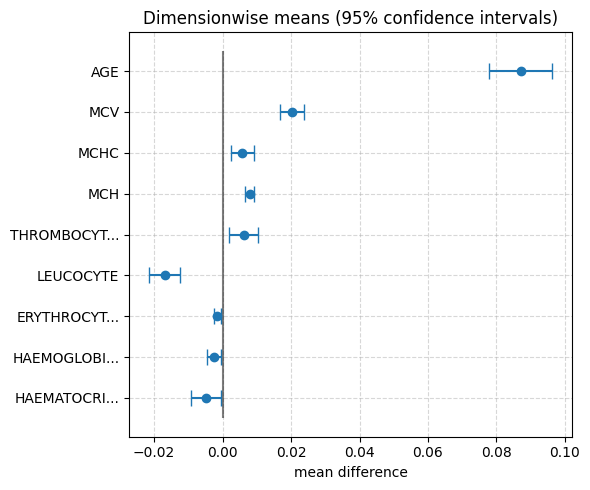
\includegraphics[width=0.7\textwidth]{images/begeat_dimension.png}
    \caption{Dimensionwise Means Difference for BeGreat Model}
    \label{fig:begreat_means_diff}
\end{figure}

From Figure \ref{fig:begreat_means_diff}, Model BeGreat shows small mean differences for most dimensions, with the largest difference observed in AGE. The overall pattern indicates a close match to the original data for most dimensions, suggesting good accuracy in replicating the original data's means.

\begin{figure}[H]
    \centering
    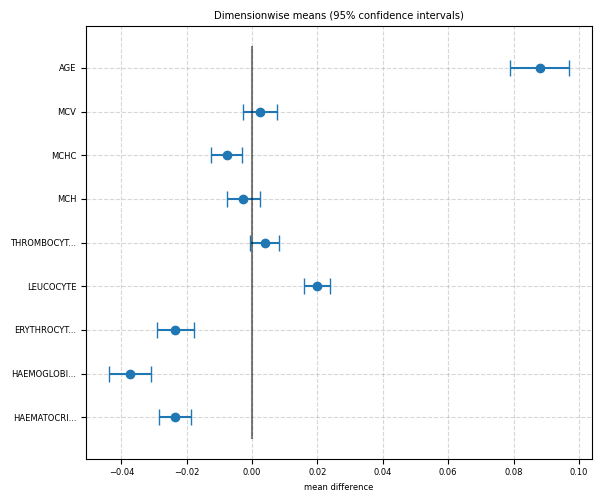
\includegraphics[width=0.7\textwidth]{images/ctgan_dimension.png}
    \caption{Dimensionwise Means Difference for CTGAN Model}
    \label{fig:ctgan_means_diff}
\end{figure}

From Figure \ref{fig:ctgan_means_diff}, Model CTGAN shows small mean differences for most dimensions, but with slightly larger differences in dimensions like AGE and MCV. The overall pattern indicates a reasonable match to the original data for most dimensions, though not as close as BeGreat.

\begin{figure}[H]
    \centering
    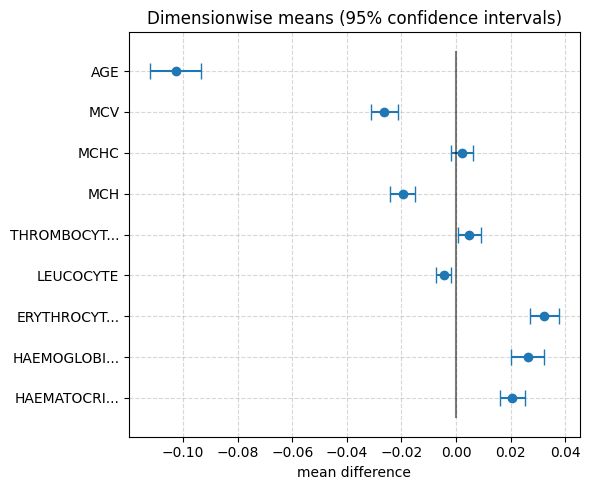
\includegraphics[width=0.7\textwidth]{images/llama_dimension.png}
    \caption{Dimensionwise Means Difference for Llama3 Model}
    \label{fig:llama3_means_diff}
\end{figure}

From Figure \ref{fig:llama3_means_diff}, Model Llama3 shows larger mean differences for several dimensions, particularly AGE, indicating a less accurate replication of the original data's means compared to BeGreat and CTGAN. However, it still demonstrates a reasonable level of accuracy for some dimensions.

\subsection{Summary of Findings}

The dimensionwise means difference plots reveal that:
- **BeGreat** shows the smallest mean differences for most dimensions, indicating the best overall performance in replicating the original data's means.
- **CTGAN** performs reasonably well but shows slightly larger differences in some dimensions compared to BeGreat.
- **Llama3** exhibits larger mean differences for several dimensions, particularly AGE, indicating a lower accuracy in replicating the original data's means.

\subsection{Conclusion}

These findings highlight the strengths and limitations of each model in terms of dimensionwise means difference. The BeGreat model is recommended for applications requiring high fidelity in replicating the original data's means, while the CTGAN model offers a balanced performance. The Llama3 model may require further refinement to improve accuracy in replicating the original data's means.


%--------------------------------------------------------------------------------------------------------------------------------------------------------------------------------------------------------------------



%--------------------------------------------------------------------------------------------------------------------------------------------------------------------------------------------------------------------


%-------------------------------------------------------------------------------------------------------------------------------------------------------------------------------------------------------------------------------------------------------------------------------------------

















% Anaylse the impact of different hyperparameters on data quality and realism.

% Discuss the ethical and societal implications of synthetic data generated using LLMs.